\documentclass{article}
\usepackage[utf8]{inputenc}
\usepackage{polski}
\usepackage[polish]{babel}
\usepackage{bbm}
\usepackage{amsmath}
\usepackage{amsthm}
\usepackage{graphicx}
\usepackage{epstopdf}
\usepackage{float}

\newtheorem{defi}{Definicja}
\newtheorem{twr}{Twierdzenie}
\newtheorem*{dd}{Dowód}

\DeclareMathOperator{\sign}{sign}
\DeclareMathOperator{\arctg}{arctg}

\newcommand{\twopartdef}[4]
{
	\left\{
		\begin{array}{ll}
			#1 & \mbox{dla } #2 \\
			#3 & \mbox{dla } #4
		\end{array}
	\right.
}


\author{Jarosław Dzikowski 273233}
\date{Wrocław, \today}
\title{\textbf{Pracownia z analizy numerycznej} \\ Sprawozdanie do zadania \textbf{P.3.11}}
\begin{document}
\maketitle
\section{Uwagi techniczne}
Program można uruchomić normalnie z wiersza poleceń. Nie wypisuje on dużo, ponieważ wyniki doświadczeń są zamieniane na wykresy. Program ma zakomentowane wywołania funkcji produkującej dane do sporządzenia wykresu przez gnuplot'a.\\

Sprawozdanie należy kompilować z wiersza poleceń będąc wewnątrz katalogu doc.
Do skompilowania sprawozdania wymagana jest obecność folderu ,,wykresy'' z wykresami w formacie eps, które następnie będą zamieszczone w sprawozdaniu. Folder ,,wykresy'' znajduje się w folderze ,,doc''.

\section{Wstęp}
W tym zadaniu zbadamy metodę Romberga całkowania numerycznego. Zbadamy jej zachowanie oraz porównamy jej rezultaty z innymi metodami.


\section{Wprowadzenie}
Zagadnienie całkowania nie jest nikomu obce. Często chcielibyśmy policzyć wartość jakiejś całki, lecz nie zawsze jest to takie proste.
Funkcja może być zbyt trudna do scałkowania lub możemy chcieć scałkować wiele funkcji, których wzorów oraz przedziałów całkowania nie znamy zawczasu.
Wtedy musimy skorzystać z jakiejś uniwersalnej metody obliczania przybliżonej wartości całki. Jedną z takich metod jest metoda Romberga.

\subsection{Kwadratury liniowe}
Zacznijmy od wprowadzenia pojęcia kwadratury. Niech $\mathbbm{F} = \mathbbm{F}[a,b]$ będzie zbiorem funkcji całkowalnych w przedziale [a,b].
Jeśli $f$ jest ciągła w [a,b), to $f \in \mathbbm{F}$. \\
Jeśli $f$ jest funkcją ograniczoną i ma skończenie wiele punktów nieciągłości w [a,b], to $f \in \mathbbm{F}$.
Całka $I: \mathbbm{F} \to \mathbbm{R}$ jest funkcjonałem liniowym.
\begin{equation*}
	I(f) = \int_a^b f(x) dx
\end{equation*}
W przypadku całki z daną funkcją wagową $p$ mamy
\begin{equation*}
	I_p(f) = \int_a^b p(x) f(x) dx
\end{equation*}
Oczywiście, z własności całki wiemy, że $I$ spełnia następujące właśności:
\begin{equation*}
	(1) \ I(f + g) = I(f) + I(g)
\end{equation*}
\begin{equation*}
	(2) \ I(\alpha f) = \alpha I(f)
\end{equation*}
\begin{defi}[Kwadratura liniowa]
	Funkcjonał $Q_n: \mathbbm{F} \to \mathbbm{R}$ postaci
	\begin{equation}
		Q_n(f) = \sum_{k = 0}^n A_k f(x_k),
	\end{equation}
	gdzie $A_k \in \mathbbm{R}$, oraz $x_0, x_1, ..., x_n \in [a,b]$ są parami różnymi punktami,
	nazywamy kwadraturą liniową. $A_k$ nazywamy współczynnikami kwadratury, natomiast $x_k$ węzłami kwadratury.
\end{defi}
Kwadratura jest zdefiniowana za pomocą $A_k$ i $x_k$. Każda kwadratura $Q_n$ jest w pewnym stopniu oddalona od całki.
\begin{defi}[Reszta kwadratury]
	Resztą kwadratury $Q_n$ nazywamy
	\begin{equation}
		R_n(f) = I(f) - Q_n(f)
	\end{equation}
\end{defi}
Niektóre kwadratury potrafią dawać dokładne wyniki całkowania dla wielomianów pewnego stopnia.
Dlatego wprowadzono pojęcie rzędu kwadratury.
\begin{defi}[Rząd kwadratury]
	Powiemy, że $Q_n$ jest rzędu $r$, jeśli
	\begin{equation*}
		i) \ \forall_{q \in \Pi_{r-1}} Q_n(q) = I(q)
	\end{equation*}
	\begin{equation*}
		ii) \ \exists_{q \in \Pi_r} Q_n(q) \neq I(q)
	\end{equation*}
\end{defi}
Każda kwadratura ma swoje limity i nie potrafi dokładnie scałkować każdego wielomianu.
\begin{twr}[Maksymalny rząd kwadratury]
	Rząd kwadratury $Q_n$ nie przekracza $2n + 2$.
\end{twr}
\begin{dd}
	\normalfont
	Niech $w(x) = [(x - x_0)(x - x_1) ... (x - x_n)]^2 \in \Pi_{2n + 2}$. Mamy
	\begin{equation*}
		Q_n(w) = \sum_{k = 0}^n A_k w(x_k) = 0 \neq I(w) = \int_a^b w(x) dx > 0
	\end{equation*}
	Podaliśmy przykład wielomianu stopnia $2n + 2$, dla którego kwadratura $Q_n$ nie osiąga dokładnej wartości całki.
	\qed
\end{dd}


\subsection{Kwadratury interpolacyjne}
Jak już wiemy, kwadratury zależą od doboru współczynników ${A_k}$ oraz węzłów ${x_k}$ kwadratury.
Co gdyby zamiast całkować funkcję $f$ spróbować scałkować wielomian interpolujący tę funkcję?
Ponieważ wielomian interpolujący jest swego rodzaju przybliżeniem $f$, liczymy na to, że całka z tego wielomianu będzie bliska całce z funkcji $f$.
\begin{defi}[Kwadratura interpolacyjna]
	Kwadraturą interpolacyjną nazwiemy kwadraturę $Q_n$, taką że
	\begin{equation*}
		Q_n(f) = I(L_n),
	\end{equation*}
	gdzie $L_n$ jest wielomianem interpolacyjnym stopnia $\leq n$ dla funkcji $f$.
\end{defi}
Wiemy, czym jest kwadratura interpolacyjna. Niestety dalej nie znamy jej współczynników ani węzłów.

\begin{twr}[Współczynniki oraz węzły kwadratury interpolacyjnej]
	Niech $L_n$ będzie n-tym wielomianem interpolacyjnym dla funkcji $f$ wyrażającym się wzorem
	\begin{equation*}
		L_n = \sum_{k = 0}^n f(x_k) \lambda_k
	\end{equation*}
	Wtedy $Q_n$ wyraża się wzorem
	\begin{equation*}
		Q_n = \sum_{k = 0}^n A_k f(x_k)
	\end{equation*}
	gdzie
	\begin{equation*}
		A_k = \int_a^b \lambda_k(x) dx = \int_a^b \left ( \prod_{\substack{j = 0 \\ j \neq k}}^n \frac{(x - x_j)}{(x_k - x_j)} \right ) dx
	\end{equation*}
	a $x_k$ są węzłami interpolacji wielomianu $L_n$.
\end{twr}
\begin{dd}
	\normalfont
	Ponieważ $Q_n(f) = I(L_n)$, wiemy, że $Q_n(L_n) = I(L_n)$, więc
	\begin{equation*}
		Q_n(L_n) = I(L_n) = \int_a^b  \sum_{k = 0}^n f(x_k) \lambda_k(x)  dx =
	\end{equation*}
	\begin{equation*}
		= \sum_{k = 0}^n f(x_k) \int_a^b \lambda_k(x) dx
	\end{equation*}
	\qed
\end{dd}

\begin{twr}[]
	$Q_n$ jest kwadraturą interpolacyjną wtedy i tylko wtedy, gdy rząd $Q_n$ jest równy co najmniej $n + 1$.
\end{twr}
\begin{dd}
	\normalfont
	$\implies$ :\\
	$Q_n(f) = I(L_n[f])$. Jeśli $f \in \Pi_n$, to $f = L_n[f]$. Stąd mamy rząd przynajmniej n + 1. \\
	$\impliedby$ :\\
	Niech $A_k$ będą współczynnikami $Q_n$, a $x_k$ węzłami $Q_n$ i $Q_n$ ma rząd $r \geq n + 1$. Zdefiniujemy $\lambda_k$ w sposób następujący
	\begin{equation*}
		\lambda_k = \prod_{\substack{j = 0 \\ j \neq k}}^n \frac{(x - x_j)}{(x_k - x_j)} \in \Pi_n
	\end{equation*}
	Zatem $Q_n(\lambda_k) = I(\lambda_k)$.
	Weźmy dowolne $f$. $L_n = \sum_{k = 0}^n f(x_k) \lambda_k$ interpoluje $f$ w węzłach kwadratury.
	$Q_n(f) = \sum_{k = 0}^n A_k f(x_k)$. Całka z $\lambda_k$ okazuje się być równa k-temu współczynnikowi kwadratury $Q_n$.
	\begin{equation*}
		I(\lambda_k) = Q_n(\lambda_k) = \sum_{j = 0}^n A_j \lambda_k(x_j) = A_k
	\end{equation*}
	Znając $A_k$ możemy wstawić je do wzoru na $Q_n(f)$.
	\begin{equation*}
		Q_n(f) = \sum_{k = 0}^n A_k f(x_k) = \sum_{k = 0}^n I_n(\lambda_k) f(x_k) = I(L_n[f])
	\end{equation*}
	Skoro $Q_n(f) = I(L_n[f])$, to $Q_n$ jest kwadraturą interpolacyjną.
	\qed
\end{dd}

\subsection{Kwadratury Newtona-Cotesa}
Kwadratury interpolacyjne, tak samo jak wielomiany interpolacyjne, zależą od doboru węzłów interpolacji.
Kwadratury Newtona-Cotesa używają najprostszych węzłów - węzłów równoodległych.
\begin{defi}[Kwadratura Newtona-Cotesa]
	Kwadraturą Newtona-Cotesa nazywamy kwadraturę interpolacyjną o węzłach równoodległych.
	\begin{equation*}
		Q_n^{NC}(f) = \sum_{k = 0}^n A_k f(x_k)
	\end{equation*}
	gdzie $x_k = a + k h, h = \frac{b - a}{n}$, $A_k = \int_a^b \lambda_k(x) dx$.
\end{defi}
Okazuje się, że dla kwadratur Newtona-Cotesa, współczynniki $A_k$ da się zapisać nieco inaczej
\begin{twr}[Współczynniki kwadratury Newtona-Cotesa]
	Niech $h = \frac{b - a}{n}$ będzie odległością między sąsiednimi węzłami.
	Wtedy współczynniki $A_k$ kwadratury Newtona-Cotesa $Q_n^{NC}$ wyrażają się wzorem
	\begin{equation*}
		A_k = h \cdot (-1)^{n - k} \cdot \frac{1}{k! (n-k)!} \cdot \int_a^b \left ( \prod_{\substack{j = 0 \\ j \neq k}}^n \frac{(x - x_j)}{(x_k - x_j)}\right ) dt
	\end{equation*}
\end{twr}
\begin{dd}
	\normalfont
	Dowód dorzucę jeśli trzeba, było na ćwiczeniach.
	\qed
\end{dd}

Dowodzi się, że błąd kwadratur Newtona-Cotesa wyraża się następująco
\begin{equation*}
	R_n(f) = \twopartdef {\frac{f^{(n + 1)}(\xi)}{(n+1)!} \int_a^b p_{n + 1}(x) dx} {2\not| n} {\frac{f^{(n + 2)}(\eta)}{(n+1)!} \int_a^b x \ p_{n + 1}(x) dx} {2 | n}
\end{equation*}
gdzie $p_{n+1}(x) = (x - x_0) (x - x_1) ... (x - x_n)$. \\
\textbf{Wniosek: }Kwadratura Newtona-Cotesa $Q_n^{NC}$ jest rzędu $\twopartdef {n + 1} {2\not| n} {n + 2} {2 | n}$.

Najbardziej znaną kwadraturą Newtona-Cotesa jest ta dla $n = 1$. $Q_1^{NC}$ z węzłami $x_0 = a, x_1 = b$, $h = b - a$ nazywamy \emph{wzorem trapezów}.
Mamy $A_0 = A_1 = \frac{h}{2}$.
\begin{equation}
	T(f) = Q_1^{NC}(f) = \frac{b - a}{2} [f(a) + f(b)]
\end{equation}
Za pomocą wzoru trapezów jesteśmy w stanie poprawnie scałkować każdą funkcję stałą oraz liniową.
Błąd wzoru trapezów $R_1(f)$ jest równy
\begin{equation*}
	R_1(f) = \frac{f''(\xi)}{2} \int_a^b (x - a)(x - b) dx = - \frac{(b - a)^3}{12} f''(\xi)
\end{equation*}

Dla $n = 2$ otrzymujemy \emph{wzór Simpsona}:
\begin{equation*}
	h = \frac{b - a}{2}, \ x_0 = a, \ x_1 = \frac{a + b}{2}, \ x_2 = b,
\end{equation*}
\begin{equation*}
	A_0 = A_2 = \frac{h}{3}, \ A_1 = 4 \frac{h}{3}
\end{equation*}
\begin{equation}
	S(f) = Q_2^{NC}(f) = \frac{b - a}{6}[f(a) + 4f\left(\frac{a + b}{2}\right) + f(b)]
\end{equation}
Rząd wzoru Simpsona wynosi 4, więc możemy poprawnie scałkować nawet wielomian trzeciego stopnia.
Błąd wzoru Simpsona wynosi
\begin{equation*}
	R_2(f) = \frac{f^{(4)}(\eta)}{4!} \int_a^b x \cdot \left(x - a\right)\left(x - \frac{a+b}{2}\right)\left(x - b\right) dx =
\end{equation*}
\begin{equation*}
	= - \frac{1}{90} \left(\frac{b - a}{2} \right)^5 f^{(4)}(\eta) = - \frac{h^5}{90} f^{(4)}(\eta)
\end{equation*}

Wykazuje się, że istnieją takie funkcje ciągłe, dla których ciąg kwadratur Newtona-Cotesa nie jest
zbieżny do całki $\int_b^a f$. Między innymi z tego powodu nie stosuje się w praktyce kwadratur Newtona-Cotesa wyższych
rzędów. Na ogół bardziej celowy jest podział przedziału całkowania $[a, b]$ na $n$ równych podprzedziałów
$[t_k, t_{k+1}]$, wyznaczony przez punkty $t_k = a + kh (k = 0, 1, \ldots , n)$, gdzie $h = \frac{b - a}{n}$, a następnie
zastosowanie w każdym z nich kwadratury Newtona-Cotesa niskiego rzędu. Otrzymujemy w ten sposób
\emph{kwadratury złożone} Newtona-Cotesa, służące do obliczania całki w całym przedziale $[a, b]$.\\
Jeśli w każdym z podprzedziałów $[t_k, t_{k+1}]$ użyć wzoru trapezów
\begin{equation*}
	\int_{t_k}^{t_{k + 1}} f(x) dx = \frac{h}{2}[f(t_k) + f(t_{k + 1})] - \frac{h^3}{12} f^{\prime\prime}(\xi_k),
\end{equation*}
gdzie $\xi_k \in (t_k,t_{k + 1})$, to otrzymamy
\begin{equation*}
	\int_a^b f(x) dx = \sum_{k = 0}^{n - 1} \int_{t_k}^{t_{k + 1}} f(x) dx = T_n(f) + R_n^T(f),
\end{equation*}
gdzie $T_n$ jest kwadraturą nazywaną \emph{złożonym wzorem trapezów}, określoną wzorem
\begin{equation*}
	T_n(f) = h {\sum_{k = 0}^n} {}^{\prime\prime} f(t_k),
\end{equation*}
gdzie $\sum {}^{\prime}$ oznacza sumę z pierwszym składnikiem podzielonym przez dwa, a $
sum {}^{\prime\prime}$ oznacza sumę z pierwszym i ostatnim składnikiem podzielonym przez dwa. \\
$R_n^T$ jest resztą tej kwadratury, równą
\begin{equation*}
	R_n^T(f) = -\frac{h^3}{12} \sum_{k = 0}^{n - 1} f^{\prime\prime}(\xi_k) = - n \frac{h^3}{12} f^{\prime\prime} (\xi) = -(b - a)\frac{h^2}{12} f^{\prime\prime} (\xi)
\end{equation*}
dla pewnego $\xi \in (a,b)$, pod warunkiem, że $f \in C^2[a,b]$.\\
Niech n będzie liczbą parzystą, $n = 2m$. Załóżmy, że $f \in C^4[a,b]$ i podzielmy przedział całkowania
na $m$ podprzedziałów $[t_k, t_{k + 1}]$ o długości $2h$, a następnie zastosujmy do całki w każdym
podpzedziale wzór Simpsona
\begin{equation*}
	\int_{t_{2k}}^{t_{2k + 2}} f(x) dx = \frac{2h}{6}[f(t_{2k}) + 4 f(t_{2k + 1}) + f(t_{2k + 2})] - \frac{h^5}{90} f^{(4)} (\eta_k),
\end{equation*}
gdzie $\eta_k \in (t_{2k}, t_{2k + 2})$. W efekcie otrzymujemy
\begin{equation*}
	\int_a^b f(x) dx = \sum_{k = 0}^{m - 1} \int_{t_{2k}}^{t_{2k + 2}} f(x) dx = S_n(f) + R_n^S(f),
\end{equation*}
gdzie $S_n(f)$ jest \emph{złożonym wzorem Simpsona}:
\begin{equation*}
	S_n(f) = \frac{h}{3}[f(t_0)\ + 4 f(t_1)\ + 2f(t_2)\ + 4f(t_3)\ + 2f(t_4)\ + \ldots\ + 2f(t_{2m - 2})\ + 4f(t_{2m - 1})\ + f(t_{2m})] =
\end{equation*}
\begin{equation*}
	= \frac{h}{3}[2 \sum_{k = 0}^m {}^{\prime\prime} f(t_{2k}) + 4 \sum_{k = 1}^m f(t_{2k - 1})],
\end{equation*}
a $R_n^S(f)$ jest resztą tego wzoru
\begin{equation*}
	R_n^S(f) = - \frac{h^5}{90} \sum_{k = 0}^{m - 1} f^{(4)}(\eta_k) = - m \frac{h^5}{90} f(\eta) = -(b - a) \frac{h^4}{180} f^{(4)} (\eta),
\end{equation*}
gdzie $\eta \in (a,b)$. \\
Ze wzorów na reszty złożonych wzorów trapezów i Simpsona wynika, że dla dostatecznie regularnych funkcji $f$ całka $I(f)$ może być przybliżona
dowolnie blisko za pomocą $T_n(f)$ lub $S_n(f)$, pod warunkiem, że weźmiemy dostatecznie małe $h$. Zachodzi zatem
\begin{equation*}
	\lim_{n \to \infty} T_n(f) = \lim_{n \to \infty} S_n(f) = I(f)
\end{equation*}
\\
Problemem dla kwadratur Newtona-Cotesa są funkcje, dla których przedział całkowania nie zawiera się w dziedzinie funkcji.
Przykładem jest następująca całka $\int_{-1}^1 \frac{1}{\sqrt{1 - x^2}} dx$ Ponieważ w punktach $x = -1$ oraz $x = 1$ funkcja jest nieokreślona,
nie możemy zastosować kwadratur Newtona-Cotesa.

\section{Metoda Romberga}
W tej sekcji posłużymy się poznanymi już złożonymi kwadraturami Newtona-Cotesa do wyprowadzenia metody Romberga
całkowania numerycznego.
\subsection{Twierdzenie Eulera - Maclaurina}
Oznaczmy przez $B_k$ k-tą liczbę Bernouliego. Przypomnijmy:
\begin{equation*}
	\frac{x}{e^x - 1} = \sum_{n = 0}^\infty \frac{B_n}{n!} x^n
\end{equation*}

\begin{defi}[Twierdzenie Eulera - Maclaurina]
	Niech $f \in C^{2m + 2}[a,b]$. Wtedy reszta złożonego wzoru trapezów wyraża się wzorem
	\begin{equation}
		R_n^T(f) = \frac{c_1}{n^2} + \frac{c_2}{n^4} + \frac{c_3}{n^6} + \ldots + \frac{c_m}{n^{2m}} + \frac{d(n)}{n^{2m + 2}} \; (n \to \infty),
	\end{equation}
	gdzie $d(n)$ jest funkcją ograniczoną, tzn. $\exists_{M} \forall_{n} |d(n)| < M$ oraz
	\begin{equation*}
		c_k = \frac{(b - a)^{2k}}{(2k)!} B_{2k} [f^{(2k - 1)}(b) - f^{(2k - 1)}(a)]
	\end{equation*}
\end{defi}

Sprawdźmy na jakimś przykładzie, jak bardzo potrafimy przyspieszyć zbieżność metody trapezów. Niech $f(x) = \frac{1}{x},\ a = 1,\ b = 3$.
\begin{equation*}
	I(f) = \int_a^b \frac{1}{x} dx = \ln 3 \approx 1.098612
\end{equation*}
Teraz policzmy tę samą całkę złożoną metodą trapezów dzieląc przedział całkowania na 64 podprzedziały.
Wydawałoby się intuicyjne, że jeśli podzielimy przedział całkowania na dwa razy więcej przedziałów,
to uzyskamy dużo lepszy wynik. Niestety okazuje się, że tak nie jest.
\begin{equation*}
	T_{64} = \textbf{1.0986}85 \quad T_{128} = \textbf{1.0986}30
\end{equation*}
Złożona metoda trapezów dla podwojonej liczby przedziałów nie dała większej liczby cyfr dokładnych.
Spójrzmy na błąd złożonej metody trapezów przy podziale na $n$ przedziałów
\begin{equation*}
	R_n^T(f) = \frac{c_1}{n^2} + \frac{c_2}{n^4} + \ldots + \frac{d(n)}{n^{2m + 2}} \quad\quad R_n^T = I - T_n
\end{equation*}
A następnie na błąd przy podziale na $2n$ przedziałów
\begin{equation*}
	R_{2n}^T(f) = \frac{c_1}{4n^2} + \frac{c_2}{16n^4} + \ldots  \quad\quad R_{2n}^T = I - T_{2n}
\end{equation*}
Spróbujmy usunać $\frac{c_1}{n^2}$ - najbardziej znaczący ze składników reszty $R_n^T(f)$
\begin{equation*}
	4R_{2n}^T(f) - R_n^T(f) = -\frac{3}{4} c_2 \frac{1}{n^4} - \frac{15}{16} c_3 \frac{1}{n^{16}} - \ldots \quad\quad 4R_{2n}^T - R_n^T = 3I - (4T_{2n} - T_n)
\end{equation*}
Zatem dla
\begin{equation*}
	T_n^\prime = \frac{4T_{2n} - T_n}{3}
\end{equation*}
zachodzi
\begin{equation*}
	R_n^\prime = I - T_n^\prime = - \frac{c_2}{4n^4} - \frac{5}{16n^6} + \ldots
\end{equation*}
Sprawdźmy teraz, jaki efekt otrzymamy w porównaniu do wcześniej wyliczonych $T_{64}$ i $T_{128}$.
\begin{equation*}
	T_{64}^\prime = \frac{4T_{128} - T_{64}}{3} = \textbf{1.098612}...
\end{equation*}
Widać, że zwiększyliśmy liczbę cyfr dokładnych.

\subsection{Tablica Romberga}
Skoro udało nam się wyeliminować najbardziej znaczący składnik błędu złożonego wzoru
trapezów $R_n^T$, to dlaczego mielibyśmy zatrzymać się w tym miejscu? W analogiczny sposób jak poprzednio możemy usunąć
kolejny najbardziej znaczący składnik reszty: $\frac{1}{n^4}$. Następnie możemy usuwać kolejne najbardziej znaczące
składniki. W ten właśnie sposób działa metoda Romberga. \\
W metodzie tej skonstruujemy trójkątną tablicę kolejnych ,,przyspieszeń" złożonego wzoru trapezów.
Niech
\begin{equation*}
T_{0,k} = T_{2^k}
\end{equation*}
Pierwsza kolumna tablicy wypełniona jest złożonymi wzorami trapezów dla podziału
przedziału całkowania na $2^k$ równych części. Niech $h_k = \frac{b - a}{2^k}$ oznacza długośc podprzedziału. \\
Kolejne kolumny tablicy konstruujemy poznaną przez nas metodą:
\begin{equation}
	T_{m,k} = \frac{4^m T_{m - 1, k + 1} - T_{m - 1, k}}{4^m - 1}
\end{equation}
W efekcie otrzymujemy następującą tablicę:

\begin{table}[h]
\centering
\begin{tabular}[c]{|c c c c c c|}
\hline
$T_{0,0}$ &  &  &  &  & \\
$T_{0,1}$ & $T_{1,0}$ &  &  & & \\
$T_{0,2}$ & $T_{1,1}$ & $T_{2,0}$ & & & \\
$T_{0,3}$ & $T_{1,2}$ & $T_{2,1}$ & $T_{3,0}$ &  &  \\
\dots & \dots & \dots & \dots & \dots & \\
$T_{0,k}$ & $T_{1,k - 1}$ & $T_{2,k - 2}$ & $T_{3,k - 3}$ & \dots & $T_{k,0}$ \\
\hline
\end{tabular}
\caption{Tablica Romberga.}
\end{table}

\begin{twr}[Druga kolumna tablicy Romberga]
	W drugiej kolumnie tablicy Romberga znajdują się złożone wzory Simpsona dla $n = 2^i, (i = 0, 1, \ldots)$, tj.
	\begin{equation*}
		T_{1, k} = S_{2^{k+1}}
	\end{equation*}
\end{twr}
\begin{dd}
	\normalfont
	Niech $n = 2m$. Rozwińmy wzór na $S_n$.
	\begin{equation*}
		S_n(f) = \frac{h}{3}[f(t_0)\ + 4 f(t_1)\ + 2f(t_2)\ + 4f(t_3)\ + 2f(t_4)\ + \ldots\ + 2f(t_{2m - 2})\ + 4f(t_{2m - 1})\ + f(t_{2m})] =
	\end{equation*}
	\begin{equation*}
		= \frac{h}{3}[2 \sum_{k = 0}^m {}^{\prime\prime} f(t_{2k}) + 4 \sum_{k = 1}^m f(t_{2k - 1})] =
	\end{equation*}
	\begin{equation*}
		= \frac{h}{3}[4 \sum_{k = 0}^m {}^{\prime\prime} f(t_{2k}) + 4 \sum_{k = 1}^m f(t_{2k - 1})] - \frac{h}{3} 2 \sum_{k = 0}^m {}^{\prime\prime} f(t_{2k}) =
	\end{equation*}
	\begin{equation*}
		= \frac{4 T_n(f) - T_m(f)}{3}
	\end{equation*}
	Widzimy, że otrzymany wzór jest taki sam jak wzór na drugą kolumnę w tablicy Romberga. Stąd
	\begin{equation*}
		S_{2^{k+1}} = \frac{4T_{2^{k+1}} - T_{2^k}}{3} = \frac{4T_{0,k+1} - T_{0,k}}{3} = T_{1,k}
	\end{equation*}
	\qed
\end{dd}

Przy obliczaniu pierwszej kolumy, czyli złożonych wzorów trapezów dla $n = 2^i$ możemy wykonać małą optymalizację,
która pozwoli nam policzyć wszystkie $T_{0,0}, T_{0,1}, \ldots, T_{0,k}$ czyli de facto $T_1, T_{2}, \ldots, T_{2^k}$
dodając wartość funkcji całkowanej w każdym z $2^k$ węzłów tylko jeden raz. Niech $h_i = \frac{b-a}{2^i}$.
\begin{equation*}
	T_{2^{i+1}} = \frac{1}{2} T_{2^i} + \frac{h_i}{2} \sum_{k = 1}^{2^i} f\left(a + k h_i - \frac{h_i}{2}\right)
\end{equation*}
W załączonym programie pierwsza kolumna tablicy Romberga obliczana jest właśnie w taki sposób.\\
Należy wspomnieć, że ponieważ w metodzie Romberga wykorzystujemy kwadratury dla węzłów równoodległych, nie możemy
scałkować funkcji, dla których przedział całkowania nie zawiera się w ich dziedzinach.

\section{Doświadczenia}
Przejdźmy teraz do prezentacji wyników doświadczeń. Zbadamy działanie metody Romberga na pięciu funkcjach.
Tak jak polecono w zadaniu, liczenie kolejnych wierszy tablicy Romberga przerwiemy w momencie, gdy dla pewnego $K > 0$
\begin{equation*}
	|T_{K,0} - T_{K-1,0}| < \epsilon |T_{K,0}|
\end{equation*}
Dodatkowo policzymy pełną tablicę Romberga oraz przedstawimy pełną tablicę błędów.
Dla każdej funkcji obliczono wartość całki za pomocą wbudowanej w Julii funkcji \verb+quadgk()+,
która oblicza całkę
używając kwadratur Gaussa-Konroda.

\begin{enumerate}
	\item $\int_a^b f(x) dx = \int_{-1}^{1} \frac{1}{x^4 + x^2 + 0.9} dx \approx 1.5822329637296728$ \\ \\
	\begin{figure}[H]
		\centering
	    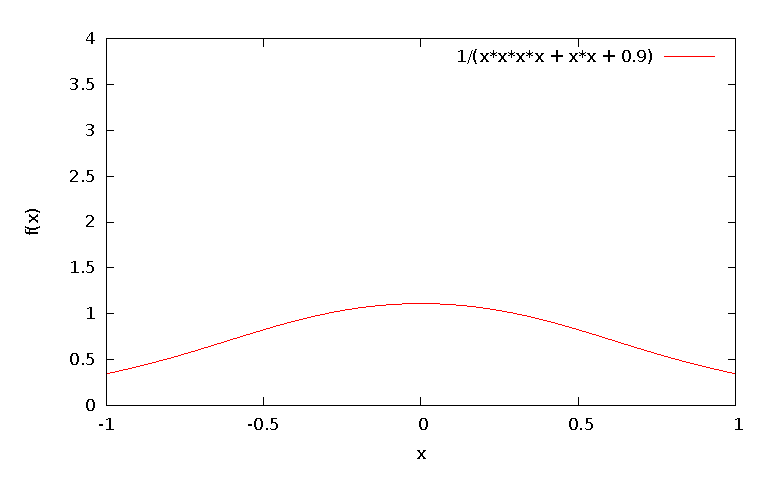
\includegraphics[width=0.8\textwidth]{wykresy/1.eps}
	    \caption{$f(x) = \frac{1}{x^4 + x^2 + 0.9}$}
	\end{figure}
	\item $\int_a^b f(x) dx = \int_0^1 \frac{1}{1 + x^4} dx \approx 0.866972987339911$ \\ \\
	\begin{figure}[H]
		\centering
		\includegraphics[width=0.8\textwidth]{wykresy/2.eps}
		\caption{$f(x) = \frac{1}{1 + x^4}$}
	\end{figure}
	\item $\int_a^b f(x) dx = \int_0^1 \frac{2}{2 + \sin(10 \pi x)} dx \approx 1.1547005383792308$ \\ \\
	\begin{figure}[H]
		\centering
		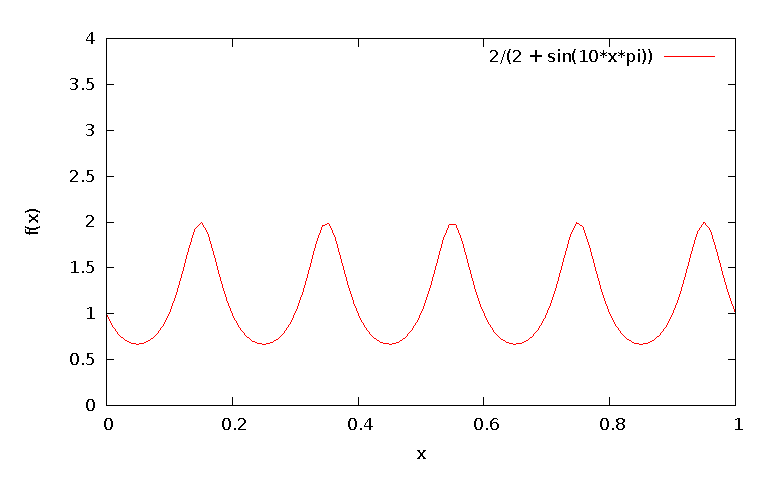
\includegraphics[width=0.8\textwidth]{wykresy/3.eps}
		\caption{$f(x) = \frac{2}{2 + \sin(10 \pi x)}$}
	\end{figure}
	\item $\int_a^b f(x) dx = \int_{-200}^{200} \cos(\frac{200}{1 + x^2}) dx  \approx 364.56214839923837$ \\ \\
		Dla tej funkcji zbyt trudno narysować wykres, ponieważ w przedziale $[-1, 1]$ cosinus ,,wariuje".
		Natomiast przy $x \to \pm \infty$ funkcja $f$ dąży do jedynki.
	\item $\int_a^b f(x) dx = \int_{-0.9999}^{0.9999} \frac{1}{\sqrt{1 - x^2}} dx \approx 3.113308146635046$ \\ \\
	\begin{figure}[H]
		\centering
		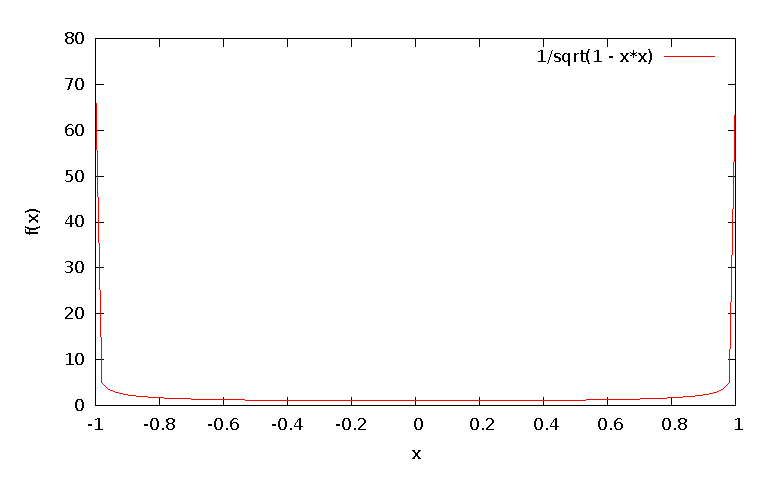
\includegraphics[width=0.8\textwidth]{wykresy/5.eps}
		\caption{$f(x) = \frac{1}{\sqrt{1 - x^2}}$}
	\end{figure}
\end{enumerate}

\section{Wnioski}

\begin{thebibliography}{9}

\bibitem{Dahlquist&Bjorck}
Dahlquist, G., Bjo\"rck, A.
\emph{Numerical Methods in Scientific Computing, Volume I},
Society for Industrial and Applied Mathematics (September 4, 2008), 354-360.

\bibitem{Cheney&Light}
Cheney, E. W., Light, W. A.
\emph{A Course in Approximation Theory},
American Mathematical Soc., 2009, 11-22.

\bibitem{Erdos}
Erdo\"s, P.
\emph{Problems and results on the theory of interpolation, II.}
Acta Math. Acad. Sci.
Hungar. 12 (1961), 235-244.

\bibitem{Brutman}
Brutman, L.
\emph{On the Lebesgue function for polynomial interpolation.}
SIAM J. Numerical Analysis 15 (1978), 694-704.

\bibitem{Rivlin}
Rivlin, T.J.
\emph{Chebyshev Polynomials}
Wiley, New York, 1974. 2nd Edition, 1990.

\bibitem{Turetskii}
Turetskii, A. H.
\emph{The bounding of polynomials prescribed at equally distributed points.}
Proc. Pedag. Inst. Vitebsk 3 (1940), 117-127.

\bibitem{Faber}
Faber, G.
\emph{Uber die interpolatorische Darstellung stetiger Funktionen.}
Jahresber. Deutsch. Math. Verein., 23 (1914), 191-200.

\bibitem{Vertesi}
Vertesi, P.
\emph{Optimal Lebesgue constant for Lagrange interpolation.}
SIAM J. Numerical Analysis Vol. 27 (1990), 1322–1331.

\end{thebibliography}

\end{document}
